\documentclass[11pt,a4paper]{article}

\usepackage[T1]{fontenc}
\usepackage[utf8x]{inputenc}
\usepackage[italian]{babel}
\usepackage{helvet}
\usepackage{multirow}
\renewcommand*\familydefault{\sfdefault}
\linespread{1.2}
\usepackage{fancyhdr}
\usepackage{lastpage}
\usepackage{graphicx}
\usepackage{tabularx}
\usepackage{hyperref}
\usepackage{float}

\usepackage[
a4paper,
top=2.5cm,
bottom=2.5cm,
left=1.5cm,
right=1.5cm,
head=30pt,
textheight=8in,
footskip=10pt
]{geometry}

\usepackage[italian]{isodate}
\usepackage{arydshln}
\usepackage{hyperref}
\usepackage{amsfonts, amsmath, amsthm, amssymb}

% Specifies custom hyphenation points for words or words that shouldn't be hyphenated at all
\hyphenation{ionto-pho-re-tic iso-tro-pic fortran} 
\hypersetup{
	colorlinks=true,
	linkcolor=black,
	urlcolor=blue
}

%----------------------------------------------------------------------------------------
%	PAGE STYLE
% ---------------------------------------------------------------------------------------
\pagestyle{fancy}
\fancyhf{}
\setlength{\headheight}{2cm} 

% Delete the paragraph indentation
\setlength{\parindent}{0pt}

%----------------------------------------------------------------------------------------
%	UNIPD STYLE
% ---------------------------------------------------------------------------------------
\newcommand{\stileUNIPD}{
	
	% header
	\lhead{
		\textline[t]{
\includegraphics[width=1cm, keepaspectratio=true]{img/UniPd.png}}
		{Progetto di Web Information Management}
		{\nomeStudente \cognomeStudente\\ (\matricolaStudente)}
	}
	
	% footer
	\rfoot{\thepage/\pageref{LastPage}} %per le prime pagine: mostra solo il numero romano
	\cfoot{}
	
}


%----------------------------------------------------------------------------------------
% 	HEADING STILE
%----------------------------------------------------------------------------------------

\newcommand\textline[4][t]{%
	\noindent\parbox[#1]{.333\textwidth}{\raisebox{-0.40\height}{#2}}%
	\parbox[#1]{.333\textwidth}{\centering #3}%
	\parbox[#1]{.333\textwidth}{\raggedleft #4}%
}

% Header delle pagine UNIPD style, commentarle se si intende usare lo stile aziendale

\stileUNIPD

% Header delle pagine stile aziendale, usaree, dopo aver chiesto il consenso all'azienda
% per l'uso del logo e dei dati personali. Commentarle se si intende usare l'UNIPD style

%\stileAziendale

% Line under the heading
\renewcommand{\headrulewidth}{0.4pt}  

%-----------------------------------------------------------------------------------------
%   FOOTER STYLE
%-----------------------------------------------------------------------------------------

%***PIÈ DI PAGINA***
%\lfoot{
\includegraphics[keepaspectratio = true, width = 25px] {img/UniPd.png} \textit{\nomeStudente 
%\cognomeStudente (\matricolaStudente)}\\ \footnotesize{\emailStudente}}
%\rfoot{\thepage/\pageref{LastPage}} %per le prime pagine: mostra solo il numero romano


\renewcommand{\footrulewidth}{0.4pt}   %Linea sopra il piè di pagina


%----------------------------------------------------------------------------------------
%   USEFUL COMMANDS
%----------------------------------------------------------------------------------------

\newcommand{\dipartimento}{Dipartimento di Matematica ``Tullio Levi-Civita''}

%----------------------------------------------------------------------------------------
% 	USER DATA
%----------------------------------------------------------------------------------------

\newcommand{\nomeStudente}{Riccardo}
\newcommand{\cognomeStudente}{Bernucci}
\newcommand{\matricolaStudente}{1121331}
\newcommand{\emailStudente}{riccardo.bernucci@studenti.unipd.it}


%----------------------------------------------------------------------------------------
% 	SITE DATA
%----------------------------------------------------------------------------------------

\newcommand{\nomeSito}{AnimeForce}
\newcommand{\linkSito}{http://www.AnimeForce.org/}



\begin{document}
	
	%Impostata la pagina iniziale
	\begin{titlepage}
	
	% Defines a new command for the horizontal lines, change thickness here
	\newcommand{\HRule}{\rule{\linewidth}{0.5mm}} 
	
	% Center everything
	\center
	
	%----------------------------------------------------------------------------------------
	%	HEADING SECTIONS
	%----------------------------------------------------------------------------------------
	
	% Name of your university/college
	\textsc{\LARGE Università degli Studi di Padova}\\[1cm] 
	
	%----------------------------------------------------------------------------------------
	%	LOGO SECTION
	%----------------------------------------------------------------------------------------
	
	
\includegraphics[height=5cm]{img/UniPd.png}\\[1cm]
	
	
\includegraphics[height=1.5cm, width = 9cm]{img/MathDip.png}\\
	\textsc{\dipartimento}\\[1.2cm]
	% Major heading such as course name
	\textsc{\Large Scuola di Scienze}\\[0.5cm] 
	
	% Minor heading such as course title
	\textsc{\large Corso di Laurea in Informatica}\\[0.5cm] 
	
	\vspace{2.5cm}
	
	%----------------------------------------------------------------------------------------
	%	TITLE SECTION
	%----------------------------------------------------------------------------------------
	
	\HRule \\[0.4cm]
	{ \huge \bfseries PROGETTO DI WEB INFORMATION MANAGEMENT}\\[0.6cm] % Title of your document
	{ \huge \emph{Analisi di usabilità di un sito web} }
	\HRule \\[1cm]
	
	%----------------------------------------------------------------------------------------
	%	AUTHOR SECTION
	%----------------------------------------------------------------------------------------
	
	\vspace{1cm}
	
	\begin{minipage}{0.5\textwidth}
		\begin{flushleft} 
			\center
			\emph{\bfseries Autore: }\nomeStudente\ \cognomeStudente\ \\
			\emph{\bfseries Matricola: }\matricolaStudente \\
			\emph{\bfseries Sito analizzato: } \linkSito \\
			\emph{\bfseries Periodo di analisi: } Marzo - Aprile 2019
		\end{flushleft}
	\end{minipage}
	
\end{titlepage}

\tableofcontents
\newpage
	
	%Analisi preliminare: presento il sito che sto per analizzare. Breve descrizione con o senza le proprie opinioni personali
	\section{Analisi preliminare}
Il sito web \nomeSito \ si pone come obiettivo quello di fornire agli appassionati di anime (ovvero video di animazione giapponese) un luogo dove poter guardare in streaming con i sottotitoli in italiano la propria serie preferita ed eventualmente poterla scaricare. Questo sito funziona come indice e database di contenuti trovati pubblicamente disponibili su Internet. L'offerta del sito è notevole perché riporta ad oggi 1252 anime e il team che ci lavora dietro continua a tenerlo aggiornato rispetto le nuove uscite. \\
Attualmente lo visito spesso, soprattutto per seguire le serie che non trovo su Netflix. Ho sempre trovato gli anime che cercavo tuttavia ha delle pecche, che andremo a vedere in questa analisi, che ne compromettono l'esperienza a livello utente.
\\
\\
La seguente analisi è stata redatta utilizzando un Lenovo Thinkpad T520 con una risoluzione di 1366x768 ed adottando il browser Google Chrome Versione 73.0.3683.86. Nel caso delle immagini per il lato mobile si è optato per l'uso degli strumenti per sviluppatori, voce di Chrome, e si è impostato un iPhone 5/SE.  

	
	%Presentare la pagina iniziale breve descrizione della metafora del negozio e presentazione 6 assi informativi
	\section{Homepage} \label{Homepage}
Un sito web lo possiamo paragonarlo ad un negozio. Prima di entrare in un nuovo negozio l’approccio comune consiste nel guardare la vetrina. Questo è un punto cruciale, perché é proprio in quel momento che decidiamo se entrare in un negozio oppure proseguire oltre. Questo avviene per il web esattamente allo stesso modo. La homepage in questo contesto é la vetrina del negozio. \\
Arrivati quindi alla vetrina bisogna fornire all'utente nel minor tempo possibile le informazioni che sta cercando o  suscitare la sua curiosità. Il proprietario del sito web deve pertanto cercare di soddisfare le cosiddette 6 W. 

\begin{figure}[H]
	\centering 
	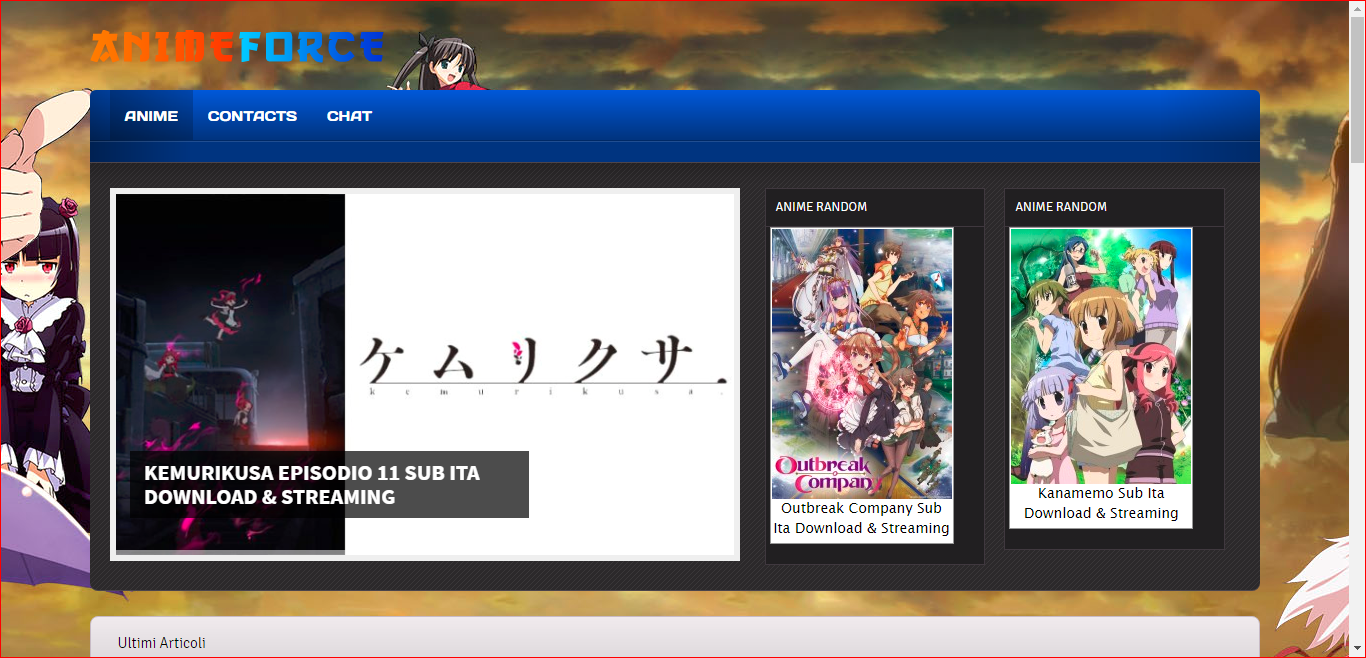
\includegraphics[width=1\textwidth]{img/homepage01.png}
	\caption{Homepage} 
	\label{img1} 
\end{figure}

\subsection{I 6 assi informativi} \label{Assi informativi}

\subsubsection{Where - "A che sito sono arrivato?"} \label{HWhere}
Appena arrivato alla homepage, ho riconosciuto in tempi non eccessivamente lunghi che il sito si occupa di fornire streaming e download di anime. Ciò è stato possibile grazie alla presenza, negli unici testi presenti, delle parole "downolad \& Streaming". In questo modo é comprensibile a primo sguardo di cosa il sito tratta, per cui se una qualunque persona fosse interessata a guardare una serie animata giapponese potrebbe continuare la navigazione nel sito.

\subsubsection{Who - "Chi c'è dietro al sito?"} \label{HWho}
Il sito è facilmente comprensibile che è riferito agli anime. Chiunque riconoscerebbe le immagini e le ricondurrebbe alla categoria generica dei cartoni animati. I tempi di comprensione da questo punto di vista sono molto rapidi. La specifica di essere giapponesi è comprensibile da una parte del nome del sito (Anime), ma soprattutto dai titoli dei cartoni in uscita e recenti presentati attraverso uno slideshow. Quindi si comprende perfettamente che il team dietro alla pagina ha una passione per gli anime e il loro scopo è diffondere cultura in questo ambito.

\subsubsection{Why - "Perché dovrei dare la mia fiducia? Che benefici mi dà?"} \label{HWhy}
La pagina non presenta alcuna descrizione della sua offerta, procede con il piazzare una lista degli anime del momento e di quelli passati. Presuppone che l'utente sia arrivato alla pagina con l'intento di guardarsi un anime, o in generale ottenere delle informazioni su di esso. Questa comportamento da parte degli ideatori del sito non attira l'utente e non fornisce alcun elemento a cui poter dare fiducia. Sebbene vi siano gli utenti che tornano alla pagina, il numero sarà sicuramente minore rispetto a quello a cui potrebbero aspirare con una descrizione nella homepage e un layout più snello di contenuti rispetto a come è adesso (vedi \hyperref[img2]{Figura \ref{img2}}).

\begin{figure}[H]
	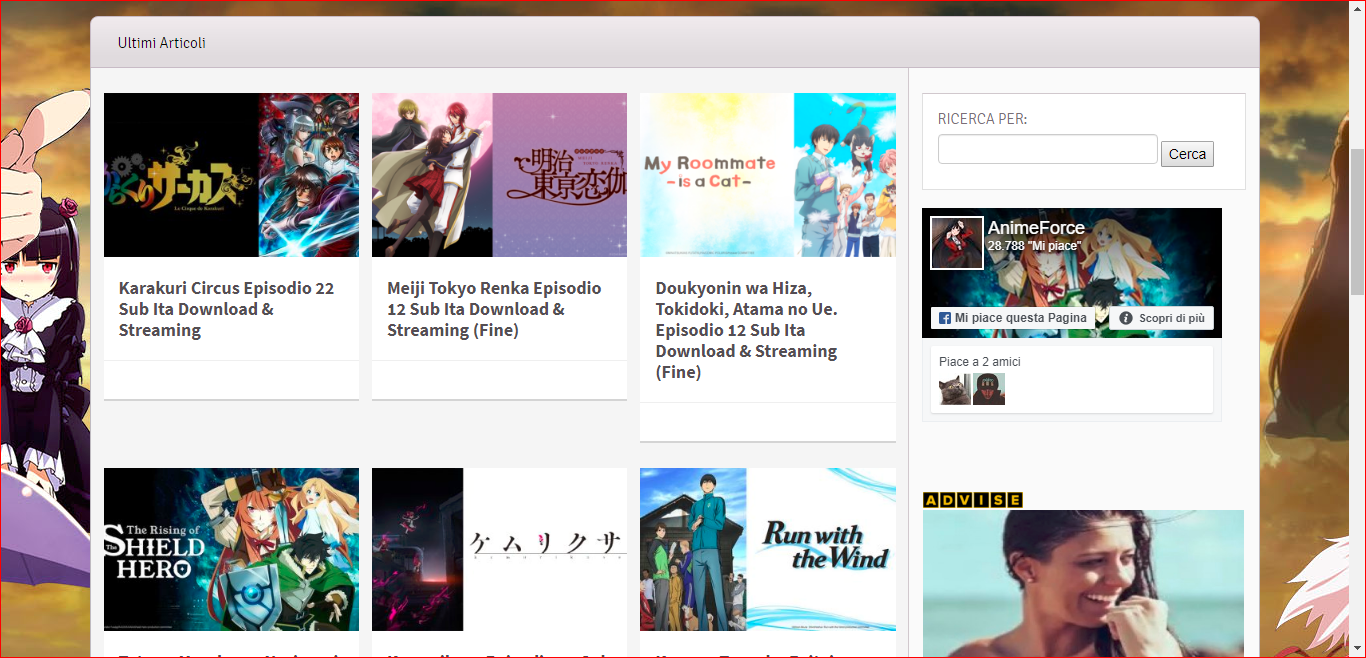
\includegraphics[width=0.5\textwidth]{img/homepage02.png}
	
\includegraphics[width=0.5\textwidth]{img/homepage03.png}
	\caption{Homepage 1 e 2 scroll} 
	\label{img2} 
\end{figure}

\begin{figure}[H]
	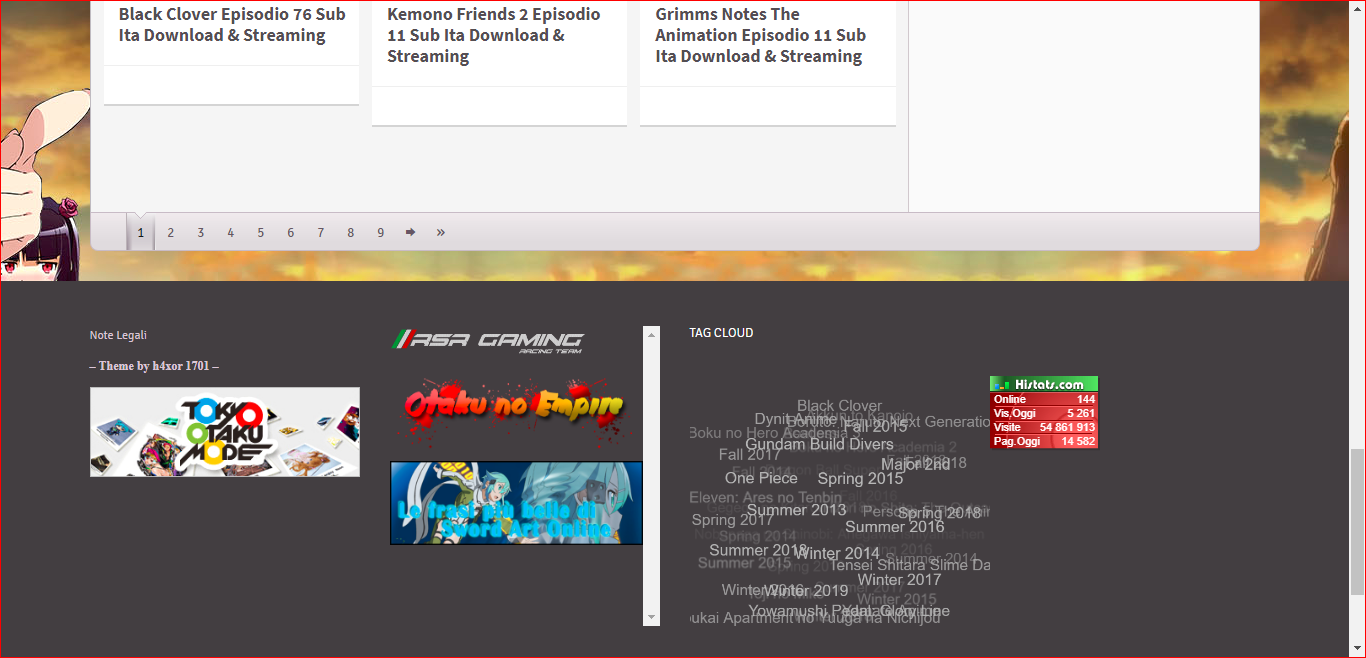
\includegraphics[width=0.5\textwidth]{img/homepage04.png}
	
\includegraphics[width=0.5\textwidth]{img/homepage05.png}
	\caption{Homepage dopo 3 e 4 scroll} 
	\label{img3} 
\end{figure}

\subsubsection{What - "Che cosa offre il sito?"} \label{HWhat}
Supponendo di aver attirato l'attenzione dell'utente; procede con effettuare degli scroll e rientrando nella dimensione di circa 2,5 pagine ha immediatamente un effetto positivo sulla pagina. Il contenuto è composto da immagini preview delle serie animate contenute nel sito in ordine di uscita, dai recenti a quelli passati. L'offerta abbiamo compreso essere un sito per streaming, ma non vi sono altre informazioni utili, quando in realtà navigando più internamente si comprende la presenza anche di informazioni quali trama, tipologia di anime e numero di serie e se vi sono nuove uscite o i "Coming soon".

\subsubsection{When - "C'è qualche novità?"} \label{HWhen}
La pagina risponde molto bene a questa domanda. Nella homepage sono presenti gli ultimi articoli inseriti e ad ogni rilascio di un nuovo episodio è possibile scoprire i contenuti nuovi.
Questo aspetto è molto importante perché permette agli utenti, soprattutto coloro che rientreranno più volte nel sito, di rimanere aggiornati e volendo anche poter ampliare le loro conoscenze su altre serie oltre a quelle che lo hanno portato a navigare sul sito \nomeSito. La manutenibilità della pagina dal punto di vista delle novità è sicuramente un punto a favore che gli permette di ottenere fiducia da parte degli utenti abituali e occasionali.


\subsubsection{How - "Come faccio ad arrivare alle sezioni principali?"} \label{HHow}
Per quanto riguarda l' "How" del sito possiamo dire che è facile ed intuitivo; utilizza il menù a tendina per la prima voce a menù (vedi figura ...) e le altre due voci, \textit{Contact} e \textit{Chat}, sono semplici link alle pagine di riferimento.
Queste voci sono posizionate in alto alla pagina e l'aspetto negativo è sicuramente che dopo aver effettuato degli scroll verso il basso spariscono. L'utente è costretto ad essere posizionato all'inizio della pagina per poter navigare usando il menù.
Oltre al menù, un altro aspetto legato al come arrivare alle principali sezioni è fornito dalla presenza di una modalità di ricerca in alto a destra e dalla seconda modalità basata sui tag a fondo pagina che risulta essere però negativa, come andremo a vedere nella sezione Ricerca (\hyperref[Ricerca]{Sezione \ref{Ricerca}}).






 
	
	%Descrivere il nome e il link adottato dal sito
	\section{Nome} \label{Nome}
Il sito ha un nome facile da ricordare e non risulta confondibile con altre parole. Si compone di due parole Anime e Force; la prima parola riconduce all'offerta del sito, mentre la seconda è una parola inglese facilmente riconducibile alla sua traduzione "forza". Le due parole insieme creano un suono piacevole ed armonioso ed iniziando con una vocale ha un impatto positivo sugli utenti. \\
Un aspetto negativo è il top-level domain "org" che rispetto al "com" o al "it" attrae meno; tuttavia, a mio parere, questo non influisce nel risultato finale perché oggigiorno non è necessario digitare il link corretto della pagina per arrivare ad essa, ma, attraverso il motore di ricerca, è sufficiente digitare il nome del sito o parole che riconducano ad esso.
	
	%Presentare tutti gli aspetti in comune delle pagine: Navigazione, Pubblicità, modalità do ricerca, Menù
	\section{Struttura generale}
Nella seguente sezione andremo ad analizzare la struttura del sito che accomunano tutte le pagine di \nomeSito. 

\subsection{Navigazione} \label{Navigazione}
Nella pagina è facilmente raggiungibile quanto si sta cercando con pochi click. Ho fatto il test per andare a cercare l'anime "Naruto Shippuden" prima attraverso la barra di ricerca, poi adottando la navigazione da menù e ci sono voluti rispettivamente 2 e 3 click. Attenzione che questo accade quando non è entrata in gioco il problema generale della pagina della pubblicità (vedi \hyperref[Pubblicità]{Sezione \ref{Pubblicità}}).
Tuttavia a seguito del fenomeno del deep linking, ovvero che i motori di ricerca reindirizzano gli utenti all'interno del sito senza passare per la homepage, i click in questione si riducono notevolmente ed entra in gioco un altro aspetto: "Quali informazioni presento delle 6 W?".
Ebbene il sito ha optato per gestire le informazioni interne nel seguente modo:
\begin{itemize}
	\item \textbf{Who:} in ogni pagina viene fornito il logo del sito;
	\item \textbf{What:} cliccando sul logo è possibile raggiungere la homepage e le informazioni della pagina raggiunta sono minimali ma adeguate (trama, categoria, tag, numero episodi ed altro);
	\item \textbf{When:} nelle pagine più interne questo aspetto viene tenuto nella colonna di destra "Ultime notizie";
	\item \textbf{Why:} non è presente nessuno slogan o descrizione che permetta di capire perché si è arrivati al sito in questione e per quale motivo dovrei dargli fiducia;
	\item \textbf{How:} nelle pagine interne non viene tenuto nessun tipo di modalità di ricerca, costringendo l'utente a navigare attraverso lo scroll ed eventualmente tornando alla homepage. 
\end{itemize}
L'ultimo aspetto è il Where. Quando si arriva ad una pagina è importante fin da subito aiutare l'utente a crearsi una mappa mentale che gli ricordi quali sono i percorsi già affrontati. Di seguito vengono presentate le tecniche e si analizza quali di queste viene adottata.

\newpage

\subsubsection{Breadcrumb}
La breadcrumb (letteralmente "briciole di pane") è una tecnica di navigazione usata nelle interfacce utente. Il suo scopo è quello di fornire agli utenti un modo di tener traccia della loro posizione nel sito. 
Esitono tre diverse tecniche:
\begin{itemize}
	\item \textbf{Location:} indica la pagina raggiunta nella gerarchia del sito;
	\item \textbf{Attribute:} mostra la categoria e gli attributi della pagina;
	\item \textbf{Path:} mostra il cammino dell'utente per giungere alla pagina, è dinamico e usa dei cookie per tenere traccia di tali informazioni.
\end{itemize}
\nomeSito\ ha optato per non fornire nessuna di queste informazioni di conseguenza l'utente non può crearsi alcuna mappa mentale del sito.

\subsubsection{Link colorati}
Uno delle convenzioni affermatesi grazie a Netscape è cambiare colore ai link già visitati. In questo sito ciò non accade. Quando si passa sopra ad un link, questo cambia colore e dopo aver visitato la pagina collegata, se si dovesse ritornare nella pagina di selezione o si incontrasse nuovamente quel link, questo non assume un colore diverso. \\
Considerando l'assenza di breadcrumb e del cambio colore, emerge come l'utente potrebbe avere difficoltà a crearsi una mappa mentale.

\subsubsection{Back button}
Rispetto ad un link diretto gli utenti prediligono il pulsante back, andando a minimizzare lo sforzo computazionale immediato piuttosto che il tempo. Il pulsante back funziona, tuttavia, come vederemo nella \hyperref[Pubblicità]{Sezione \ref{Pubblicità}}, la presenza di pubblicità molto invasiva rende all'utente l'esperienza nel sito abbastanza frustrante.
\subsection{Menù} \label{Menù}
Il menù è il primo sistema di navigazione di un sito. \nomeSito\ ha optato per posizionare il menù in alto alla pagina subito dopo il logo. Esso si compone di tre voci e, nel caso della prima, appare un menù a tendina con 4 link ad altre pagine. Il menù è minimal e la scelta è adeguata. Effettuando delle prove su di esso è possibile notare che il menù in caso si esca dalla sua area con il puntatore del mouse, permane per qualche secondo, di conseguenza l'utente inesperto non rischia di arrabbiarsi se sbaglia a puntare una voce. \\
Il problema di questo menù non è la posizione o la dimensione, ma la sua staticità. L'utente se effettua dei movimenti verso il basso perde il menù non può più navigare su di esso. L'utente può tornare in alto in due maniere: scrollando verso l'alto oppure, se si trova a fondo pagina, con un pulsante freccia visibile in \hyperref[img3]{Figura \ref{img3}}.\\
Le scelte migliori sarebbero state quelle di impostare il menù in alto in maniera fissa dopo la discesa oppure introducendo il pulsante "Back to top" nel momento stesso in cui scompaiono dallo schermo le voci.

\begin{figure}[H]
	
\includegraphics[width=1\textwidth]{img/menu.png}
	\caption{Menù} 
	\label{img4} 
\end{figure}
\subsection{Ricerca} \label{Ricerca}
Un problema fondamentale dei siti è far sì che il proprio contenuto sia trovato dagli utenti. La ricerca diviene quindi un fattore fondamentale all'interno del web. Esistono varie modalità di ricerca, prima di tutto ogni sito internet se abbastanza grande dovrebbe avere come servizio la ricerca interna. In questo caso il sito presenta un contenuto molto elevato quindi la modalità di ricerca è essenziale.
\nomeSito ha optato per la ricerca classica nella quale si inseriscono una serie di parole chiave e si preme il pulsante "Cerca" che manda in esecuzione la ricerca di tutti i contenuti collegati a quella parola.
Il problema è che tale tipo di ricerca lo si ritrova unicamente alla homepage. Le altre pagine non presentano questo strumento assai utile. Il menù non si ingrandisce, ma accetta un numero di parole infinito. Inoltre la modalità di ricerca è molto limitata perché costringe un utente a sapere cosa cercare e quindi deve andare in altri siti per decidere cosa guardare. La soluzione migliore sarebbe quella di categorizzare gli anime in base a dei tag, cosa che già avviene quando vengono creati e poi permettere una ricerca in base ad essi. 
Una modalità simile viene adottata a fondo pagina ma risulta scomoda così come è staata ideata. Sarebbe meglio togliere l'effetto grafico che è stato inserito e migliorare la modalità di ricerca statica.

\subsection{Errore 404}
L'errore 404 si verifica quando i link sono "rotti" (non esistono più). In questi casi, la cosa migliore da fare è dare altre scelte possibili all'utente, inserire una search box  e giocare sull'ironia dell'accaduto, per esempio con un’immagine divertente. Il fatto che ci si imbatta nella pagina 404 è un’esperienza negativa per l’utente, utile è dunque cercare di migliorare la situazione giocando sull'ironia della cosa, in modo tale che l’utente ne esca non con l’idea che ha perso tempo, ma che ha fatto una pausa da quello che stava cercando.  \\
Il sito ha optato per gestire l'errore eventuale come si vede nella \hyperref[img5]{Figura \ref{img5}} a destra con una barra di ricerca e una frase in inglese. Tuttavia, mancano quelli che potrebbero essere dei suggerimenti per la prossima navigazione, eventuali frasi che suscitino interesse, o la semplice ed ironica, immagine dinamica che rilassa i timer dell'utente.
\begin{figure}[H]
	\centering
	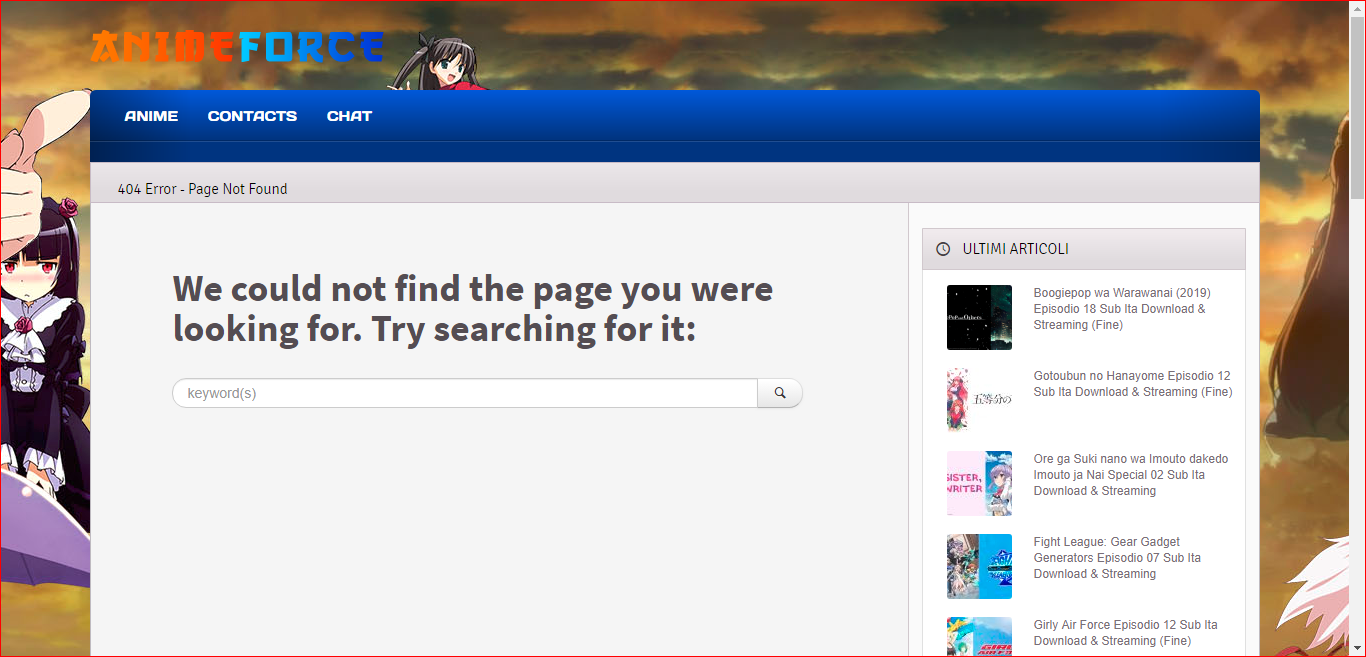
\includegraphics[width=1\textwidth]{img/Errore404.png}
	\caption{Errore 404} 
	\label{img6} 
\end{figure}
%\input{Sezioni/SitoCommerciale.tex}
\section{Pubblicità}
	
	
	%ALTRA PAGINA SCELTA: inserire i 6 assi informativi dell'altra pagina selezionata
	%la pagina deve essere una importante come ad esempio quella di un articolo o di un particolare argomento
	\section{Altra pagina del sito}

\subsection{Lista anime A-Z}

\subsection{Anime in corso}

\subsection{Anime con uscita irregolare}

\subsection{Ultime serie}

\subsection{Contacts}
	
	%FACOLTATIVO: presentare la schermata del sito in modalità mobile o tablet: come cambia, si adatta è statica vi sono problemi particolari, Qualcosa smette di funzionare...
	\section{Mobile}
	
	%Come si è deciso di gestire l'errore
	\subsection{Errore 404}
L'errore 404 si verifica quando i link sono "rotti" (non esistono più). In questi casi, la cosa migliore da fare è dare altre scelte possibili all'utente, inserire una search box  e giocare sull'ironia dell'accaduto, per esempio con un’immagine divertente. Il fatto che ci si imbatta nella pagina 404 è un’esperienza negativa per l’utente, utile è dunque cercare di migliorare la situazione giocando sull'ironia della cosa, in modo tale che l’utente ne esca non con l’idea che ha perso tempo, ma che ha fatto una pausa da quello che stava cercando.  \\
Il sito ha optato per gestire l'errore eventuale come si vede nella \hyperref[img5]{Figura \ref{img5}} a destra con una barra di ricerca e una frase in inglese. Tuttavia, mancano quelli che potrebbero essere dei suggerimenti per la prossima navigazione, eventuali frasi che suscitino interesse, o la semplice ed ironica, immagine dinamica che rilassa i timer dell'utente.
\begin{figure}[H]
	\centering
	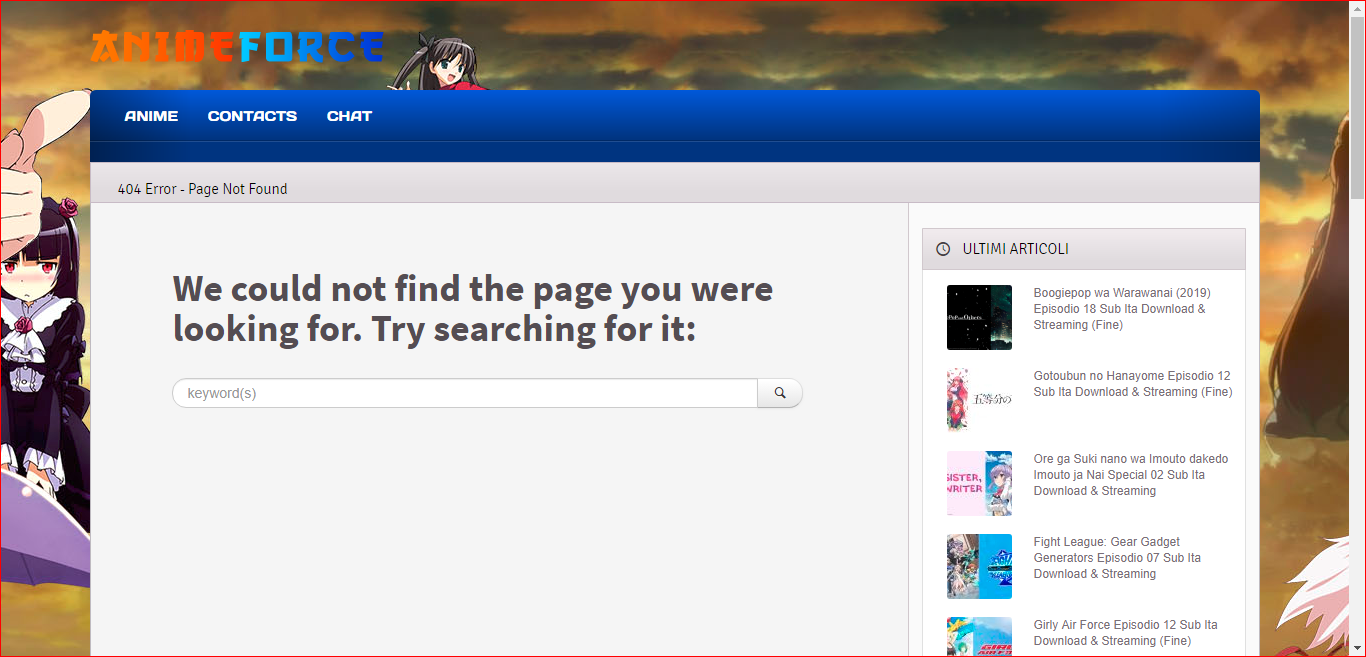
\includegraphics[width=1\textwidth]{img/Errore404.png}
	\caption{Errore 404} 
	\label{img6} 
\end{figure}
	
	%CONCLUSIONI
	\section{Conclusioni}
\begin{center}
	\begin{tabularx}{\textwidth}{|c|X|c|}
		\hline
		\textbf{Sezione} & \textbf{Valutazione} &\textbf{Voto} \\ \hline
		
		\textbf{Homepage} &	&	\textbf{6}\\
		\hdashline 
		\multirow{5}{0cm}\
		Where 	& \textit{} &	6\\
		Who		& \textit{} &	7\\
		Why 	& \textit{} &	3\\
		What 	& \textit{} &	5\\
		When 	& \textit{} &	8\\
		How 	& \textit{} &	7\\
		\hline
		
		\textbf{Nome} & \textit{\textbf{}} & \textbf{9} \\ \hline
		
		\textbf{Struttura generale} &	&	\textbf{5}\\
		\hdashline 
		\multirow{5}{0cm}\
		Navigazione & \textit{} &	2\\
		Menù		& \textit{} &	7\\
		Ricerca 	& \textit{} &	6\\
		Pubblicità 	& \textit{} &	5\\
		Errore 404	& \textit{}	&	7\\
		\hline
		 
		\textbf{Altra pagina del sito} 	& \textit{\textbf{}} & \textbf{7} \\ \hline
		\textbf{Mobile} 				& \textit{\textbf{}} & \textbf{4} \\ \hline
		
	\end{tabularx}

\end{center}

In conclusione dalla media dei voti assegnati per gli aspetti analizzati nel seguente documento, il voto del sito è di 6,20/10.
	
\end{document}